\label{desenvolvimento_processamento}

Esta seção apresenta a visão da solução da parte de processamento e interface referentes a Software, e integração com a frente de Eletro-eletrônica. A intenção desta frente é apresentar a visão da arquitetura do sistema, bem como será o fluxo de dados entre usuário até chegar ao sistema. A intenção é transmitir as decisões significativas do ponto de vista da arquitetura de baixo e alto nível que foram tomadas de acordo com as necessidades do sistema.

\subsubsection*{\textbf{Escopo}}

A arquitetura que foi idealizada fundamenta a base para a construção do produto, expressando como o sistema deverá se comportar em suas interações, bem como o nível de abrangência da aplicação em quesitos de limitação e qualidade.

O escopo deste projeto vai de encontro em cobrir os aspectos de comunicação entre usuário e sistema, bem como o tratamento dos dados embarcados. Para isso, este será apresentado o dimensionamento do sistema, tanto em alto nível, com relação à aplicação web, quanto em baixo nível, referente a rotina de comunicação entre Raspberry PI e Arduino e a rotina de processamento de dados.

\subsubsection*{\textbf{Representação da Arquitetura}}

A arquitetura da aplicação utiliza de padrões que organizam e aperfeiçoam o desenvolvimento dentro do paradigma de Orientação a Objetos e adicionalmente, a persistência e o consumo de dados.

Quanto à camada de alto nível, para o corrente projeto da bancada de vibrações, optou-se por desenvolver uma aplicação web para que o usuário possa fornecer inputs de controle para operação da bancada e também, visualizar os resultados do ensaio realizado.

É válido ressaltar que para fins de boa performance da aplicação web, foram consideradas abordagens para o projeto de aplicativos da Web fracamente acoplados. Nesse cenário, o estilo REST (Representational State Transfer - Transferência de Estado Representacional)  foi adotado.

Roy Fielding, um dos idealizadores do estilo REST,  afirma que o estilo REST enfatiza a escalabilidade das interações entre componentes e componentes intermediários para reduzir a latência da interação.

De uma forma geral, vale notar que tudo na Web (páginas, imagens, entre outros) são a essência de um recurso [1]. O fato de o REST  possuir a  característica de contar com recursos nomeados em vez de mensagens facilita o fraco acoplamento no design da aplicação.
    
Logo abaixo, é possível contemplar uma figura esquemática da arquitetura geral do sistema.

\begin{figure}[!ht]
\centering
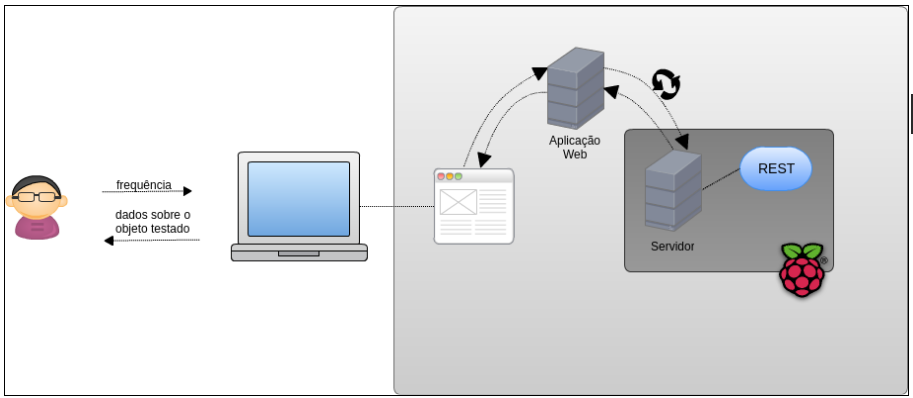
\includegraphics[scale=0.5]{figuras/arquitetura_sistema.png}
\caption{Esquema geral da arquitetura do sistema. Fonte: Autores}
\label{fig:arquitetura_sistema}
\end{figure}

Para a realização dos testes na bancada, o usuário poderá determinar a frequência de vibração e o tempo de funcionamento da bancada por meio da interação com uma aplicação web. Durante e após a execução dos testes, o usuário poderá visualizar os dados coletados pelos sensores.

A aplicação web fará requisições, através de uma rotina, para um servidor que provê serviços REST. Este servidor será disponibilizado por uma Raspberry Pi. É valido ressaltar que a comunicação entre aplicação web e o Raspberry PI funcione é necessário que o mesmo esteja com acesso a internet para que ele possa receber e enviar as requisições para a aplicação web. 

Adicionalmente, os serviços REST consultarão os dados coletados e persistidos em uma base de dados SQLite , que também será hospedado na Raspberry Pi.

Para a camada de baixo nível será desenvolvido uma rotina responsável por enviar, receber dados entre Arduino e Raspberry PI, bem como disponibilizar os dados recebidos na forma de arquivos que serão utilizados pela aplicação para que o usuário consiga ver os resultados das ações que foram aplicadas no sistema. Toda essa transmissão de dados será feita com a interface UART [2] (Universal Asynchronous Receiver Transmitter - Transmissor Receptor Assíncrono Universal), via serialização de dados.

Os dados de resultados que chegarem do Arduino para a Raspberry PI, serão tratados pela rotina de comunicação de forma a disponibilizar esses dados brutos em arquivos. Estes arquivos serão lidos por uma rotina que terá como objetivo realizar o processamento dos dados e logo em seguida a realização do parser (leitura dos dados nos arquivos e a gravação deles no banco de dados embarcado) desses dados no banco de dados local.

\begin{figure}[!ht]
\centering
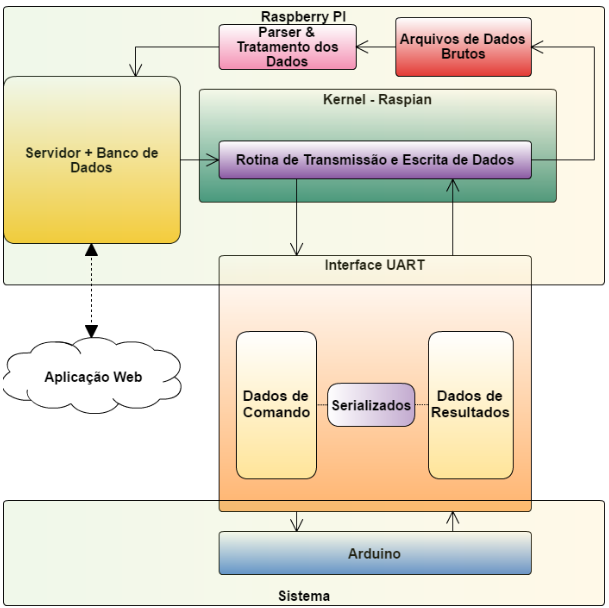
\includegraphics[scale=0.5]{figuras/sistema.png}
\caption{Camada baixo nível do sistema, responsável pela comunicação entre a aplicação web e o sistema da bancada de vibração}
\label{fig:sistema}
\end{figure}

Por fim, vale destacar que a rotina é o meio de integração entre Software e Eletrônica o qual teremos uma comunicação de baixo nível pela porta serial e os resultados obtidos entregues na forma de arquivos, ou seja, separando a comunicação entre Hardware e a aplicação. Serão utilizados rotinas para tratamento dos dados de acordo com a necessidade do usuário em visualizar os dados de resultados derivados.

\subsubsection*{\textbf{Restrições Arquiteturais}}
Com o objetivo de se criar um sistema confiável, estabeleceu-se que deverá ser feita uma avaliação dos componentes mais críticos e deverão ser elaborados testes unitários para assegurar o bom funcionamento destes módulos.

Adicionalmente, dentre as opções de linguagens de programação disponíveis para desenvolvimento de aplicações web, e do parser e tratamento dos dados brutos, optou-se pela linguagem Python e para a camada de baixo nível será utilizado a linguagem C para o desenvolvimento  das rotinas de comunicação entre Raspberry PI e Arduino. O desenvolvimento da aplicação web e dos serviços REST será feito com o auxílio de recursos providos pelo framework Django \footnotemark, que oferece uma alta produtividade no desenvolvimento.
\footnotetext{https://www.djangoproject.com/}

A linguagem de programação Python possui uma excelente performance, especialmente considerando que o hardware a ser utilizado para disponibilizar o servidor REST possui recursos de processamento bem limitados. Além disso, a linguagem de programação Python possui uma alta produtividade associada.

Outro aspecto vantajoso da linguagem é vasta disponibilidade de bibliotecas para tratamento de informações, especialmente cálculos matemáticos, que serão amplamente utilizados no sistema para uso integrado com a bancada de vibrações.

\subsubsection*{\textbf{Requisitos Levantados}}
A partir do escopo definido no projeto foram elicitados alguns requisitos de forma macro, estes podem ser vistos na Figura \ref{backlog_produto} que representa os \textit{Backlogs} do Produto para as duas aplicações.

\begin{figure}[!h]    
\centering
\label{backlog_produto}	
% 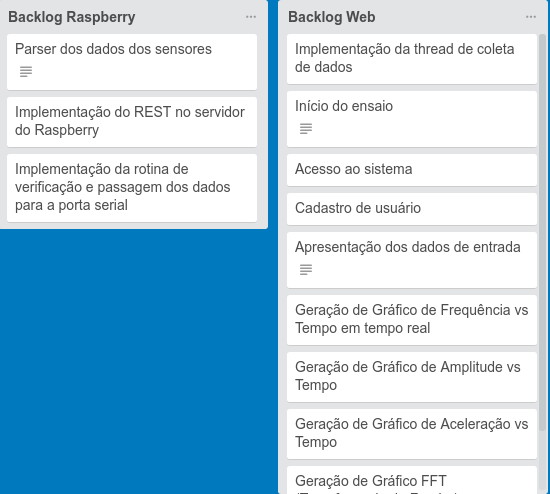
\includegraphics[keepaspectratio=true,scale=0.55]	{figuras/backlog_produto.png}
\caption{\textit{Backlogs} das aplicações do projeto}
\end{figure} 

\subsubsection*{\textbf{Protótipo da Solução Web}}

Com o intuito de visualizar a solução Web foi desenhado um protótipo de alta fidelidade da aplicação Web. As telas podem ser vistas nas Figuras \ref{fig:tela_login}, \ref{fig:tela_iniciar}, \ref{fig:tela_iniciando}, \ref{fig:tela_resultado_ensaio} e \ref{fig:tela_ensaios}.


\begin{figure}[!h]    
\centering
\label{fig:tela_login}	
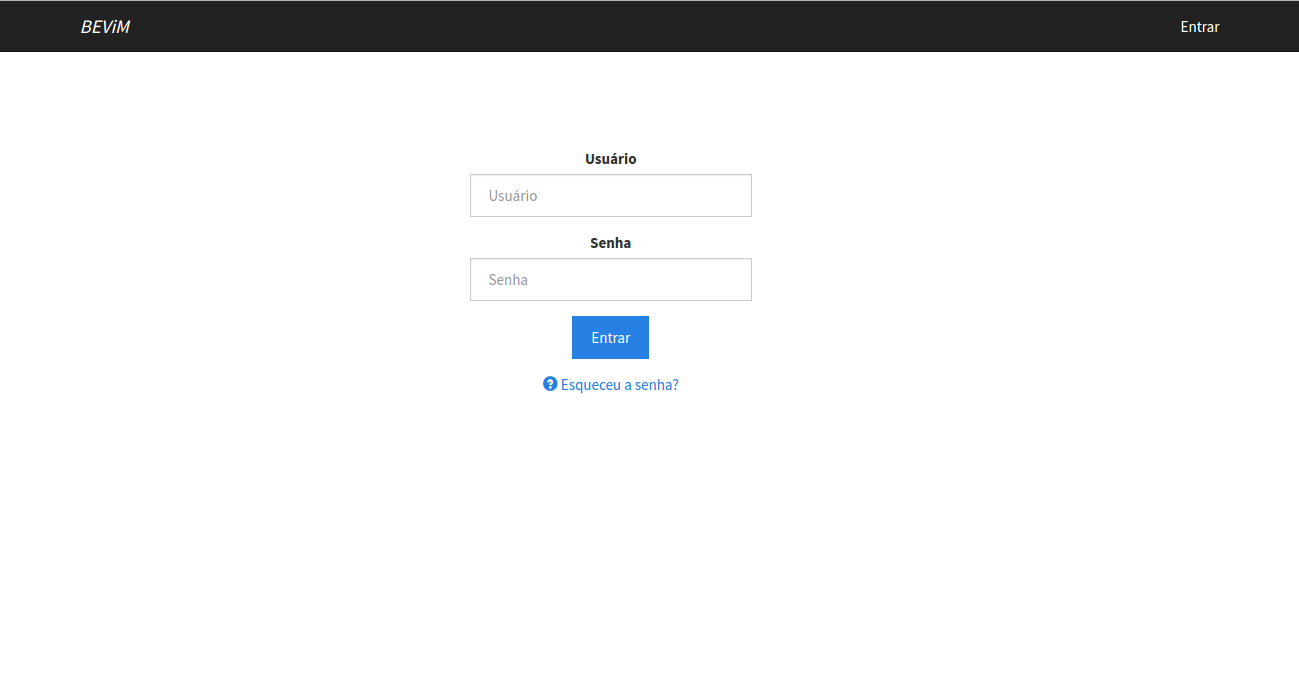
\includegraphics[keepaspectratio=true,scale=0.55]	{figuras/tela_login.png}
\caption{Tela de login da aplicação}
\end{figure}  

\begin{figure}[!h]    
\centering
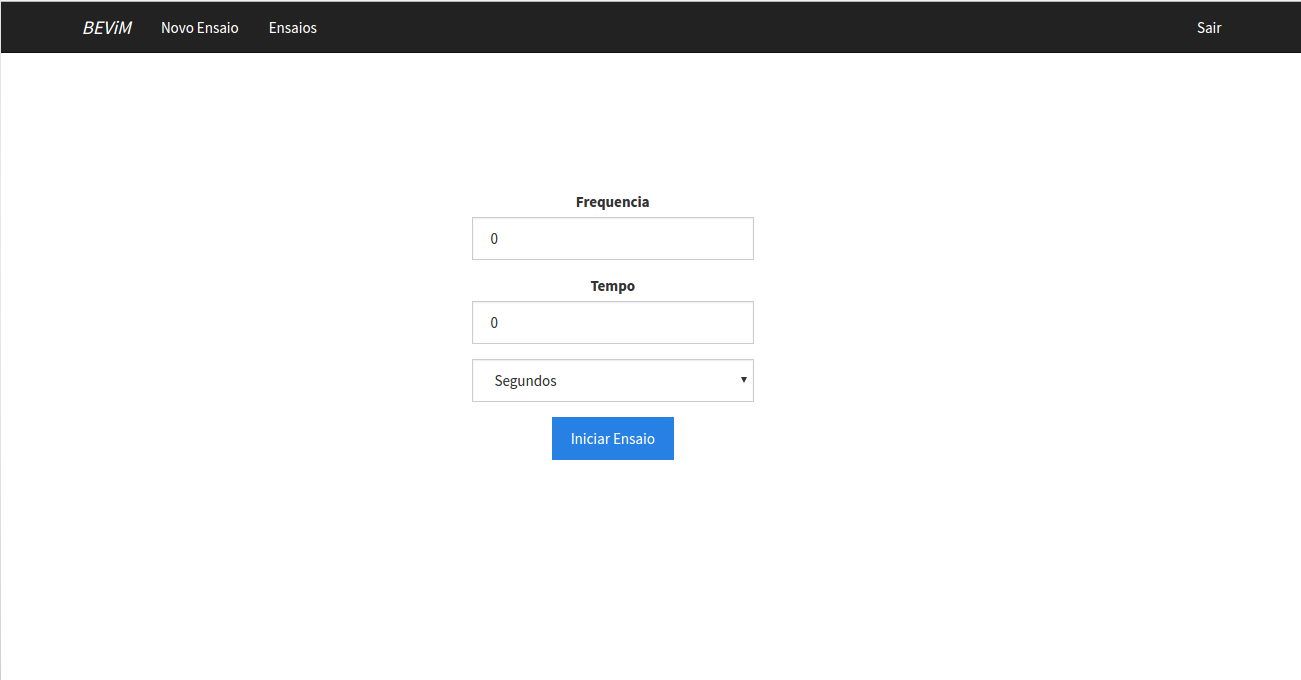
\includegraphics[keepaspectratio=true,scale=0.55]	{figuras/tela_iniciar.png}
\label{fig:tela_iniciar}	
\caption{Tela para inserir os parâmetros do ensaio}
\end{figure}  
        
\begin{figure}[!h]    
\centering
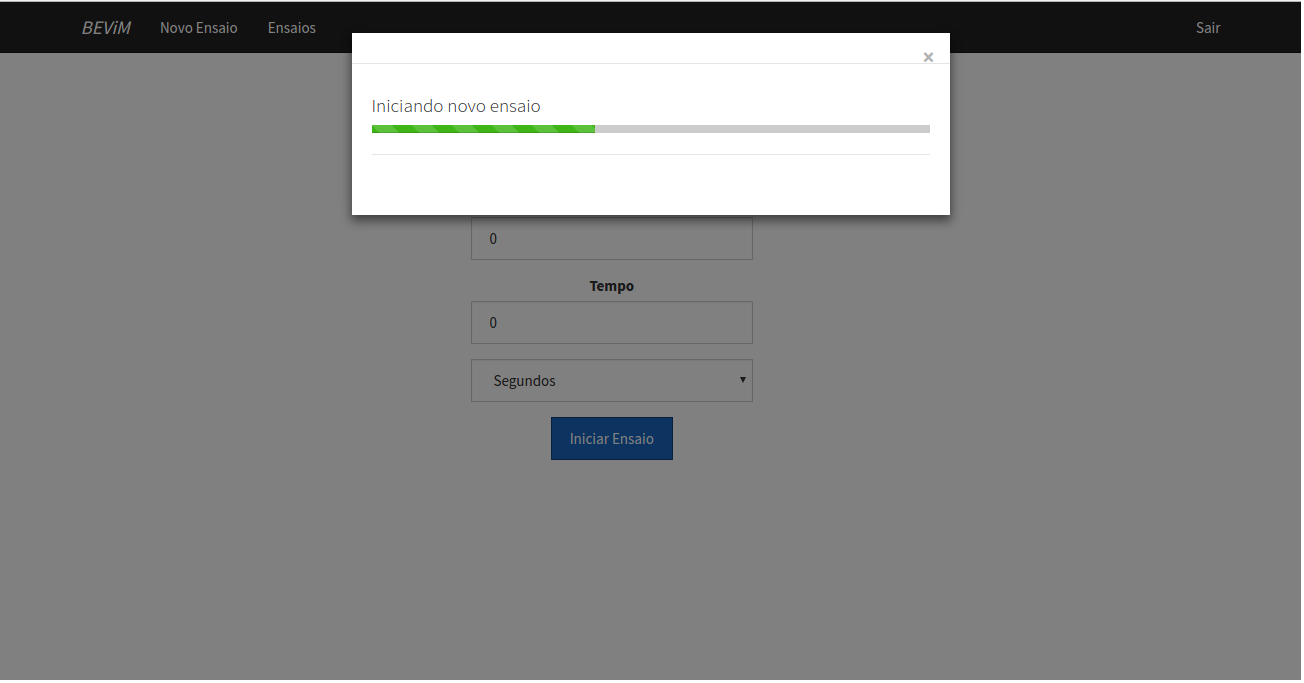
\includegraphics[keepaspectratio=true,scale=0.55]	{figuras/tela_iniciando.png}
\label{fig:tela_iniciando}
\caption{Tela referente ao processo de início do ensaio}
\end{figure}  
        
\begin{figure}[!h]    
\centering
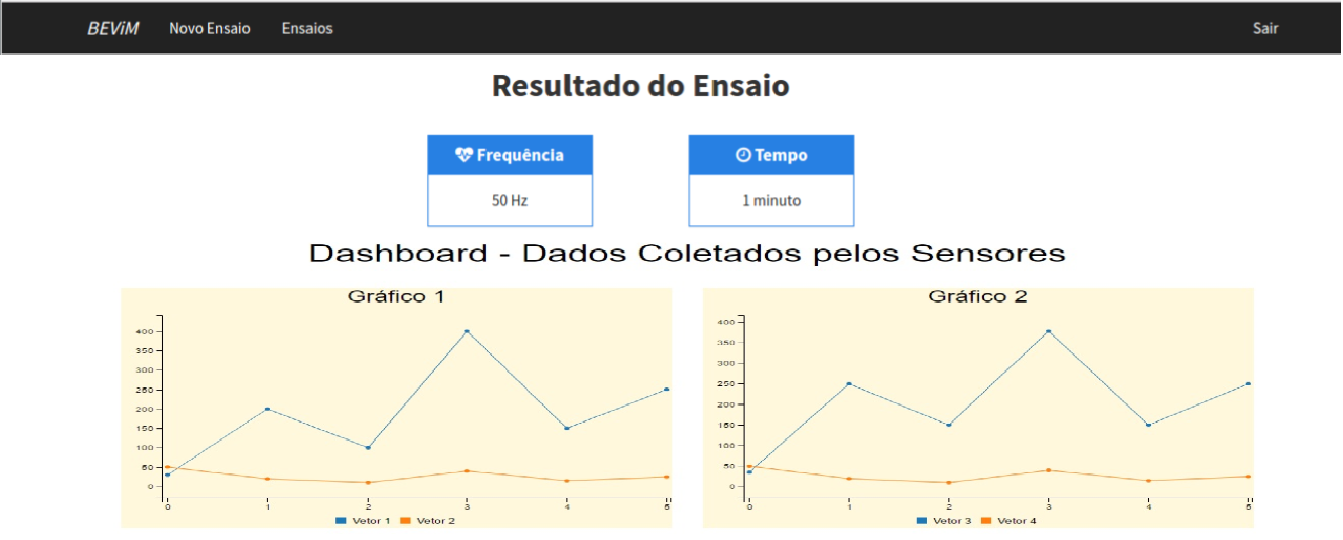
\includegraphics[keepaspectratio=true,scale=0.52]	{figuras/tela_resultado_ensaio.png}
\label{fig:tela_resultado_ensaio}	
\caption{Tela de resultados do ensaio}
\end{figure}
        
\begin{figure}[!h]    
\centering
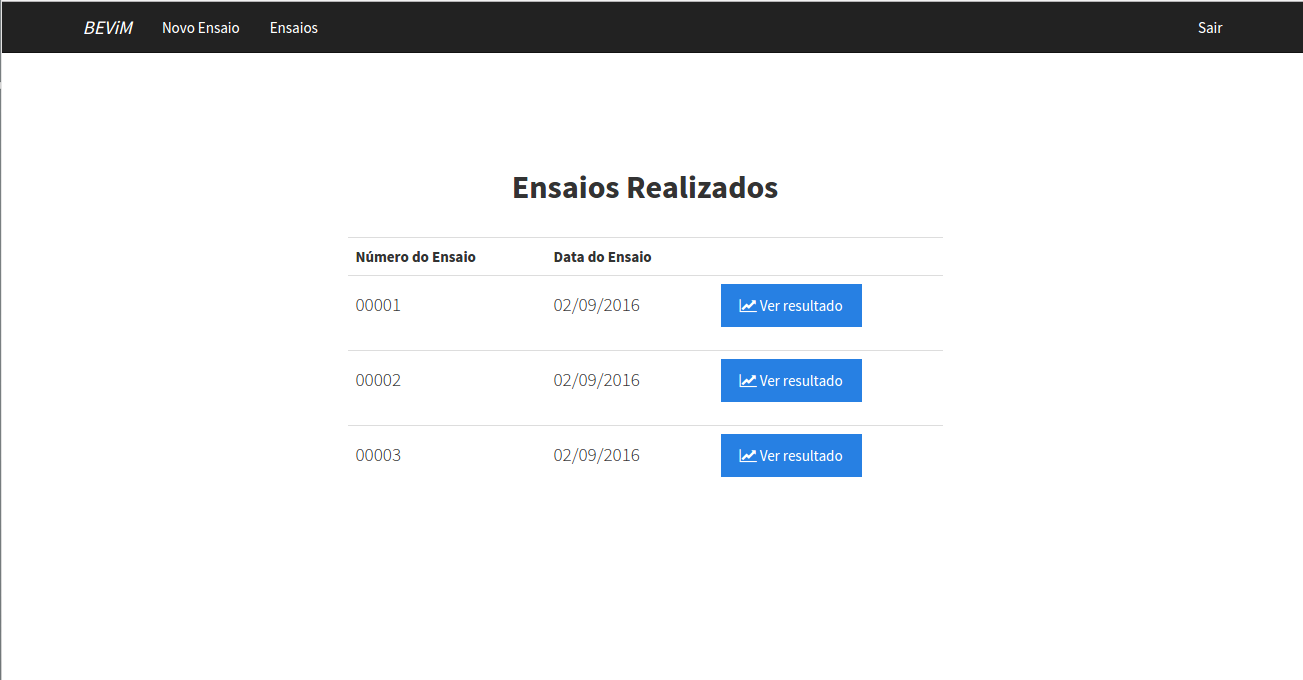
\includegraphics[keepaspectratio=true,scale=0.40]{figuras/tela_ensaios.png}
\label{fig:tela_ensaios}	
\caption{Tela dos ensaios realizados}
\end{figure}
        